% Bab IV  Hasil Penelitian dan Pembahasan
\chapter{HASIL DAN PEMBAHASAN}

\section{Hasil Penelitian}
Hasil penelitian diperoleh dari simulasi tiga algoritma penjadwalan pada lima variasi jumlah pengguna, masing-masing diulang 10 kali. Nilai yang disajikan adalah rata-rata dari 10 pengulangan. \textit{Seluruh angka pada contoh ini fiktif dan hanya memperagakan format penyajian hasil.}

\subsection{Hasil Implementasi}
Skenario pada Tabel 3.1 berhasil diimplementasikan pada ns-3 dan seluruh simulasi berjalan sampai selesai tanpa kegagalan. Satu eNodeB melayani 10 sampai 50 pengguna yang bergerak acak, dan setiap pengguna menerima aliran UDP dari server. Data \textit{throughput} setiap pengguna dicatat pada setiap simulasi dan diolah dengan Python.

\subsection{Hasil Pengukuran \textit{Throughput}}
\needspace{8cm}
Tabel 4.1 menyajikan \textit{throughput} total jaringan untuk ketiga algoritma. Pada semua jumlah pengguna, Max C/I menghasilkan \textit{throughput} tertinggi, diikuti PF, dan RR terendah. Pada 50 pengguna, PF lebih tinggi 10,2\% dan Max C/I lebih tinggi 21,9\% dibandingkan RR.

\begin{singlespace}
\begin{longtable}{|p{0.22\linewidth}|p{0.17\linewidth}|p{0.2\linewidth}|p{0.17\linewidth}|}
\caption{\textit{Throughput} total jaringan (Mbps)}\\
\hline
\textbf{Jumlah pengguna} & \textbf{RR} & \textbf{PF} & \textbf{Max C/I} \\
\hline
10 & 28,4 & 30,1 & 32,8 \\
\hline
20 & 31,2 & 34,0 & 37,5 \\
\hline
30 & 32,5 & 35,6 & 39,4 \\
\hline
40 & 33,1 & 36,4 & 40,2 \\
\hline
50 & 33,4 & 36,8 & 40,7 \\
\hline
\end{longtable}
\end{singlespace}

Kecenderungan tersebut ditunjukkan pada Gambar 4.1: \textit{throughput} meningkat seiring bertambahnya pengguna karena penjadwal memiliki lebih banyak pilihan pengguna dengan kanal baik, tetapi kenaikannya melandai pada jumlah pengguna yang besar.

\begin{figure}[H]
\centering
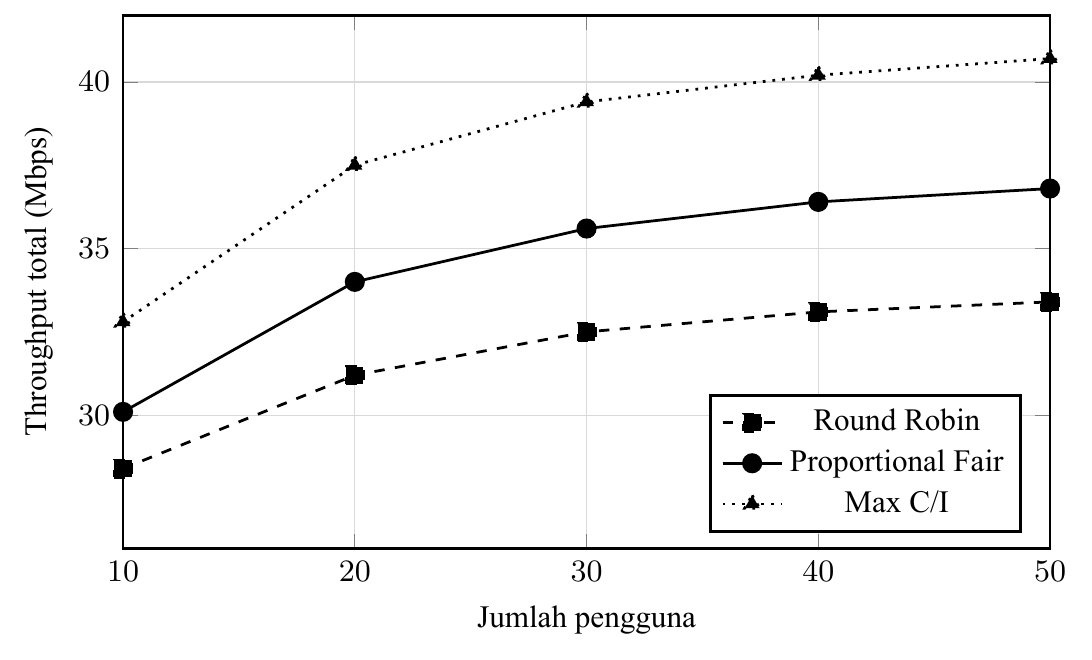
\includegraphics[width=0.62\textwidth]{../gambar/grafik-throughput.png}
\caption{Grafik \textit{throughput} total terhadap jumlah pengguna}
\end{figure}

\subsection{Hasil Pengukuran \textit{Fairness}}
\needspace{8cm}
Tabel 4.2 menyajikan indeks \textit{fairness} Jain. RR memiliki indeks tertinggi (0,90 sampai 0,93), PF berada di tengah (0,83 sampai 0,88), dan Max C/I terendah serta menurun tajam dari 0,52 menjadi 0,28 ketika jumlah pengguna bertambah (Gambar 4.2).

\begin{singlespace}
\begin{longtable}{|p{0.22\linewidth}|p{0.17\linewidth}|p{0.2\linewidth}|p{0.17\linewidth}|}
\caption{Indeks \textit{fairness} Jain}\\
\hline
\textbf{Jumlah pengguna} & \textbf{RR} & \textbf{PF} & \textbf{Max C/I} \\
\hline
10 & 0,93 & 0,88 & 0,52 \\
\hline
20 & 0,92 & 0,86 & 0,41 \\
\hline
30 & 0,91 & 0,85 & 0,35 \\
\hline
40 & 0,91 & 0,84 & 0,31 \\
\hline
50 & 0,90 & 0,83 & 0,28 \\
\hline
\end{longtable}
\end{singlespace}

\begin{figure}[H]
\centering
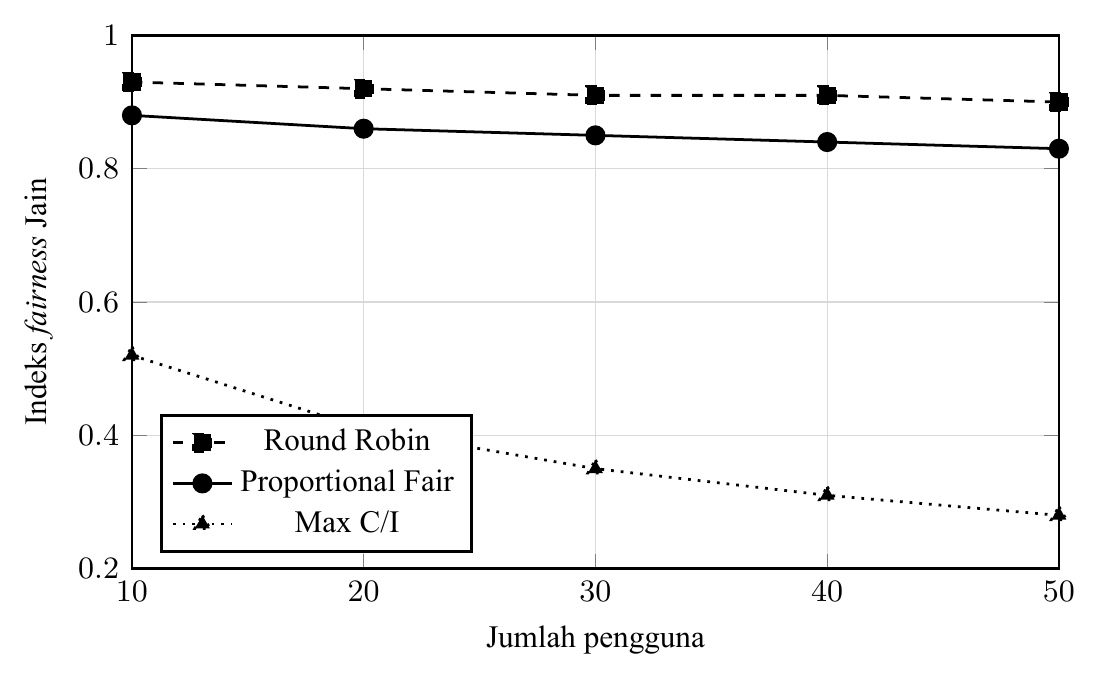
\includegraphics[width=0.62\textwidth]{../gambar/grafik-fairness.png}
\caption{Grafik indeks \textit{fairness} terhadap jumlah pengguna}
\end{figure}

\section{Pembahasan}
Hasil menunjukkan adanya \textit{trade-off} antara \textit{throughput} dan \textit{fairness}. Max C/I menghasilkan \textit{throughput} tertinggi karena sumber daya selalu diberikan kepada pengguna dengan kanal terbaik, tetapi pengguna di tepi sel jarang terlayani sehingga indeks \textit{fairness} rendah dan memburuk saat jumlah pengguna bertambah. Sebaliknya, RR membagi sumber daya secara merata sehingga adil, tetapi mengabaikan kondisi kanal sehingga \textit{throughput}-nya paling rendah.

PF memberikan kompromi: pada 50 pengguna, \textit{throughput} PF hanya 9,6\% di bawah Max C/I, sementara indeks \textit{fairness}-nya (0,83) jauh lebih tinggi daripada Max C/I (0,28), dan hanya 0,07 di bawah RR. Kecenderungan ini sesuai dengan pembahasan pada literatur bahwa Max C/I memaksimalkan efisiensi dengan mengorbankan keadilan, sedangkan PF menyeimbangkan keduanya (Capozzi et al., 2013; Andrews, 2007). Perbandingan skema penjadwalan LTE pada penelitian lain juga melaporkan perbedaan kinerja antaralgoritma (AlQahtani \& Alhassany, 2013).

Keterbatasan penelitian ini adalah simulasi hanya mencakup satu sel dengan trafik UDP konstan, sehingga hasilnya belum menggambarkan kondisi jaringan nyata dengan banyak sel dan beragam jenis trafik.
